\documentclass[11pt,a4paper]{article}
\usepackage[margin=24mm]{geometry}
\usepackage{amsmath,booktabs,graphicx,fontspec,unicode-math,hyperref}
\setmainfont{STIXGeneral}
\setmathfont{STIX Two Math}
\hypersetup{hidelinks}
\setlength{\emergencystretch}{2em}
\title{Six applications of one common theory:\\the lengths of the manuscripts}
\author{Human Compression project}
\date{11 October 2026}
\begin{document}
\maketitle
\noindent The specified main results of six historical manuscripts follow
from one common theory and six complete applications. Their mathematical
contracts have been independently reviewed and admitted in the published
edition \texttt{6641c356}. The numerical audit is separate from the
mathematical admission. All figures below bind that edition, including its final attribution
correction.

Let $c$ count NFC characters other than whitespace in the bound PDF
extractions, after the reviewed page-furniture exclusions and glyph
calibration. The comparison of written papers is
\[
 R_A=\frac{\sum_{i=1}^{6}c(L_i)}{c(U_A)+\sum_{i=1}^{6}c(A_i)}
 =\frac{195{,}379}{49{,}059+78{,}251}=1.534671\ldots.
\]
The common theory is paid in full once within this topic. Overlap with another
topic does not reduce this charge. Including the entire required program,
printed as one appendix $P$, gives the same overall comparison with that cost included:
\[
 R_{A,P}=\frac{\sum_{i=1}^{6}c(L_i)}{c(U_A)+\sum_{i=1}^{6}c(A_i)+c(P)}
 =\frac{195{,}379}{127{,}310+53{,}035}=1.083362\ldots.
\]
The four raw program files are not charged a second time.

\begin{center}\small
\begin{tabular}{llrrr}\toprule
Source & Complete application & Source & Application & Conditional\\\midrule
L032 & $A_1$: two-power orders & 16,558 & 8,212 & 2.016318\\
L034 & $A_2$: three-generator hypertopes & 21,433 & 5,784 & 3.705567\\
F016 & $A_3$: square sections and extensions & 43,983 & 15,419 & 2.852520\\
F013 & $A_4$: common two-group quotient & 25,562 & 6,224 & 4.107005\\
L035 & $A_5$: high-type two-groups & 51,019 & 14,498 & 3.519037\\
N009 & $A_6$: order-1024 markings & 36,824 & 28,114 & 1.309810\\\midrule
 & All six applications & 195,379 & 78,251 & ---\\
 & Acquisition: whole common theory & --- & 49,059 & ---\\
 & Acquisition: complete program & --- & 53,035 & ---\\\bottomrule
\end{tabular}\end{center}
Each conditional factor is $c(L_i)/c(A_i)$ \emph{after acquiring the whole
common theory and the whole complete program appendix}. It does not measure
the cost of proving that application independently. The overall comparison
charges the common theory explicitly, and its version including the program
also charges that complete appendix.

\newpage
\noindent\textbf{What is recovered and what is counted.}
The fixed contracts cover the all-parameter two-power existence theorem
(L032), the specified three-generator hypertope presentations and geometry
(L034), square sections, flatness, amalgamation and extension results
(F016), the common lower-central quotient and covering theorem (F013),
the high-type existence and complete marked classifications (L035), and
the nondegenerate order-1024 marked classification and all its comparison
tables (N009). Each contract preserves its reviewed literal corrections
and retained inputs. The particular inductive presentation and separate
classification question in L032, Question 3.3 in L034, and other statements
outside the declared contracts are not asserted to follow from this volume.
Their source text is nevertheless included in the full-manuscript numerator.

Every source page, title, abstract and bibliography is included. The
denominator contains the entire common paper, all six complete applications
and, for the second measure, the whole program appendix. There are 93 source
pages, 17 common-paper pages, 33 application pages and 21 program pages.
These physical extents are reported separately from the text coordinate.

\begin{center}
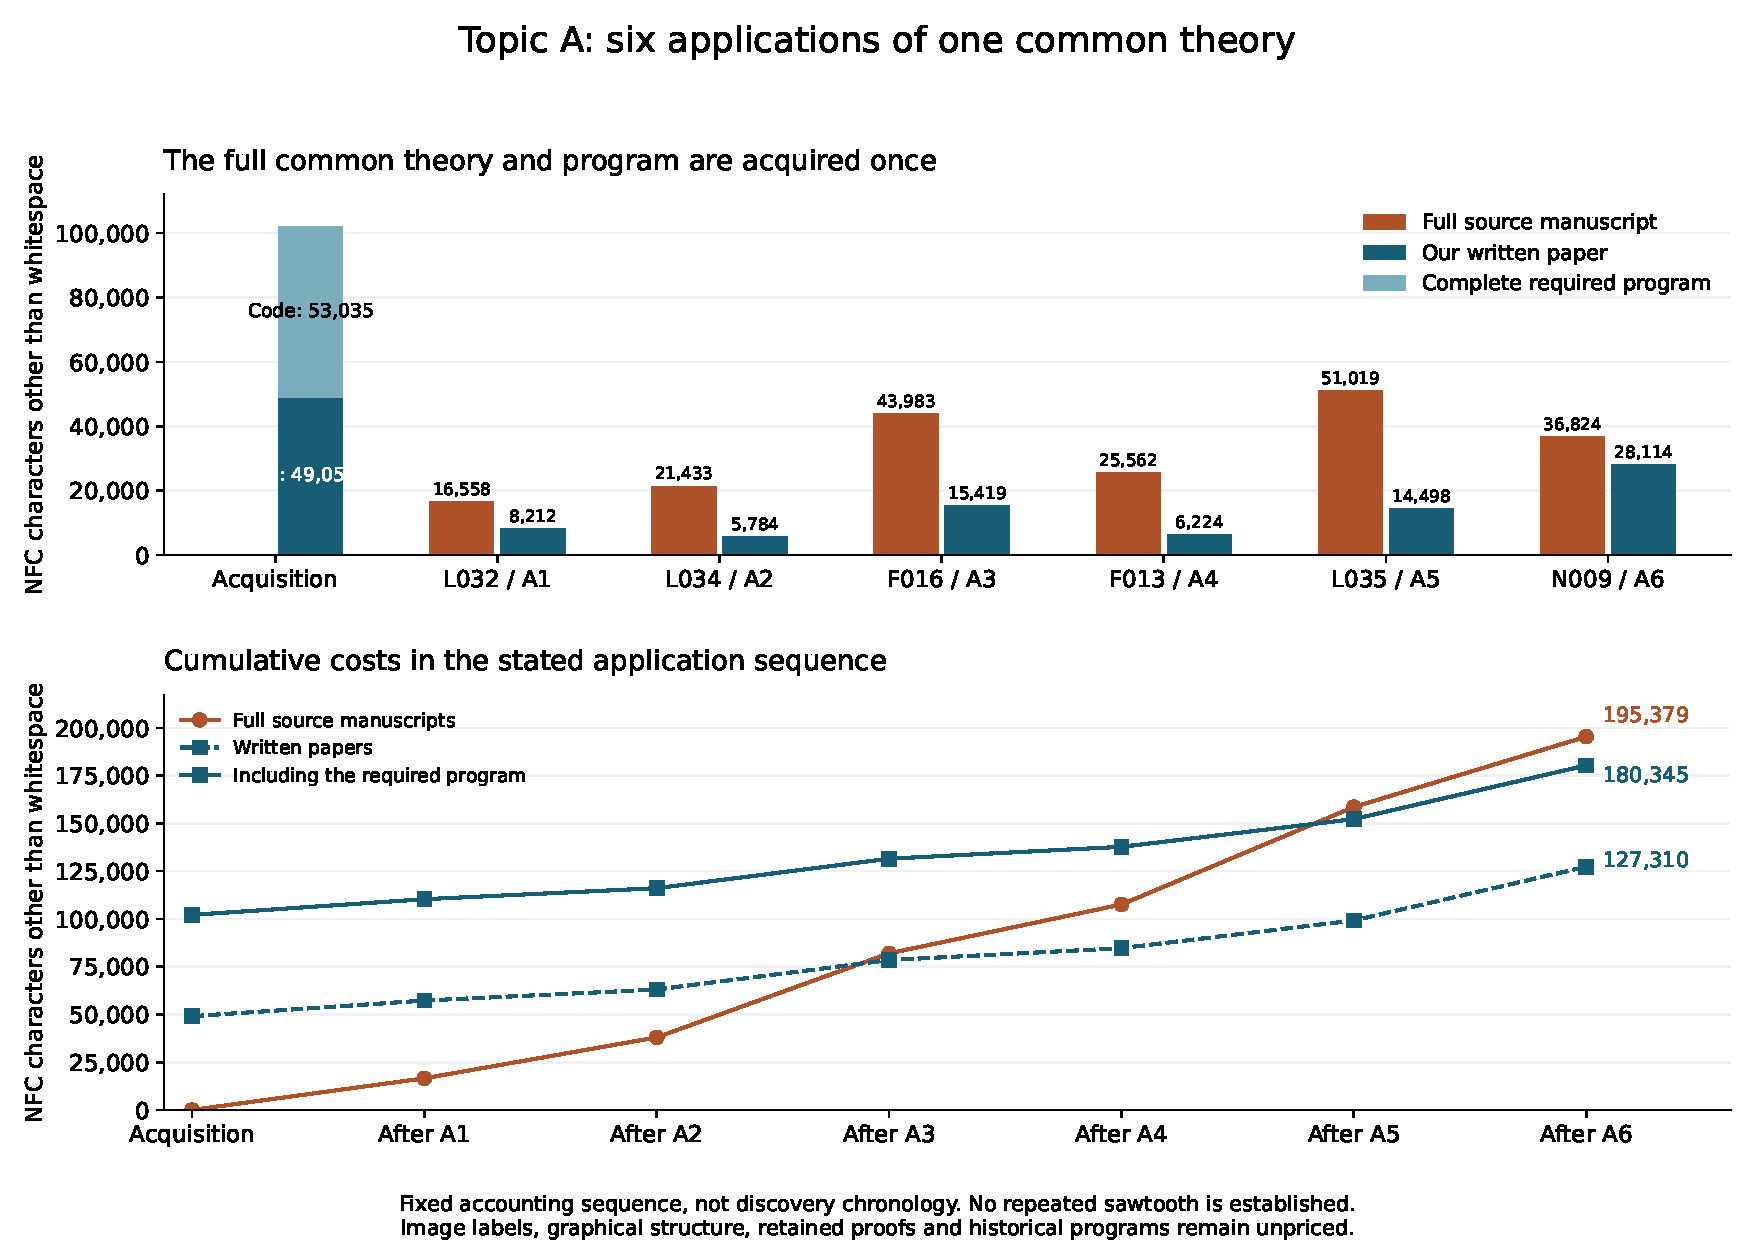
\includegraphics[width=\textwidth]{costs.pdf}
\end{center}
The plotted sequence acquires the full common theory and program before
the applications. It is an accounting order, not a chronology of discovery
or evidence of a repeated sawtooth. Historical background has not been
assigned a zero cost by the plotted starting value.

\newpage
\noindent\textbf{Metric sensitivity.}
No conversion between words, characters and bytes is presumed. Each row
uses its own unit consistently on both sides, with whole-document costs
summed without invented separators. The primary row is NFC characters
other than whitespace.
\begin{center}\small
\begin{tabular}{llrr}\toprule
Form & Unit & Written papers & Including program\\\midrule
NFC & Whitespace-separated tokens & 1.770375 & 1.556223\\
NFC & Alphanumeric units & 1.896848 & 1.444332\\
NFC & Characters other than whitespace & 1.534671 & 1.083362\\
NFC & Characters with collapsed whitespace & 1.577151 & 1.154279\\
NFC & UTF-8 bytes with collapsed whitespace & 1.488189 & 1.122995\\\midrule
NFKC & Whitespace-separated tokens & 1.772414 & 1.558015\\
NFKC & Alphanumeric units & 1.896848 & 1.444332\\
NFKC & Characters other than whitespace & 1.535608 & 1.084214\\
NFKC & Characters with collapsed whitespace & 1.578266 & 1.155246\\
NFKC & UTF-8 bytes with collapsed whitespace & 1.638395 & 1.206272\\\bottomrule
\end{tabular}\end{center}
The machine-readable record additionally retains every untrimmed and raw
selected coordinate. With no furniture removed, the primary factors are
$197{,}304/127{,}370=1.549062\ldots$ for written papers and
$197{,}304/180{,}438=1.093473\ldots$ including the program. Font-aware
calibration does not change the primary nonspace count here, but it does
change some alphanumeric and byte counts. The printed discretionary
hyphens are retained throughout.

As an alternative representation of the \emph{same} complete required
program, the four raw files contain 51,970 primary characters. Replacing
the printed appendix by those files gives $195{,}379/179{,}280
=1.089798\ldots$. The two representations are never added together.

\medskip\noindent\textbf{Limits of the measurement.}
This is a comparison of extracted text, not complete visible text. L035
pages 9, 10, 12 and 22 contain raster scientific diagrams and unextracted
labels; page 22 has no extracted text, and its embedded image is clipped.
N009 page 1 contains an image-only journal banner. Their missing labels and
graphical structure have unknown cost, not zero cost. No private image
transcription is included in these figures.

Classical group theory, geometric correspondence and the stated source
inputs remain retained. In particular, the exact infinite universal
decomposition and the specified smooth-square classification used for
N009 are not newly proved here. The full costs of retained proofs,
historical external programs, libraries and graphical constructions remain
unknown. The factors above therefore do not claim to price every artifact
needed on both sides. The separate formal scope identifies which generic
lemmas Lean verifies; neither an end-to-end formalization nor its cost is
claimed.

\medskip\noindent\textbf{Reproduction.}
The frozen numerical package supplies a portable recount with
\texttt{pypdf 6.13.0}, bound primary PDFs supplied privately, exact public
TeX/PDF/program bindings, 420 independent metric agreements and 84 text-hash
agreements. Thirteen document records retain the original independent
recount; the final A6 record was independently recounted after its
attribution correction. The two reports are preserved separately. No new
source credit, conjecture solution or priority claim follows from these
lengths.
\end{document}
